%-------------------------------------------------------------------------------
%                                PREAMBLE
%-------------------------------------------------------------------------------
\documentclass[usenames,dvipsnames,svgnames,10pt,aspectratio=169]{beamer}
%
\usefonttheme{professionalfonts}
% This theme uses TIKZ: compile twice with PDFLaTeX or LuaLaTeX.
%
%  Options:
%  - [clean]:    clean slides, i.e. logos and footbar are removed
%  - [kth]:      footbar style inspierd to the official KTH template
%  - [nicewave]: a different style of wave is used (not approved by FLOW)
%
\usetheme[clean]{flow}

\usepackage{tikz}
\usetikzlibrary{arrows}
\usetikzlibrary{shapes.geometric,math}

\usepackage[]{circuitikz}

\usepackage{pgfplots}
\usepgfplotslibrary{polar}

\usepackage{hyperref,graphicx,lmodern}
\usepackage[utf8]{inputenc}
\usepackage{media9}
\usepackage{xcolor}
\usepackage{stmaryrd}
\usepackage{nicefrac}
\usepackage{multimedia}
\usepackage{multicol}
\usepackage{upgreek}
\usepackage[]{bm}
\usepackage[]{url}
\usepackage[]{animate}
\usepackage{amsmath}

\graphicspath{{imgs/}}
\setbeamertemplate{blocks}[rounded][shadow=true]


%-------------------------------------------------------------------------------
%                                TITLE PAGE
%-------------------------------------------------------------------------------
\title[Nonlinear dynamics] % Short title used in footline
{
	First-order systems
}

\author[J.-Ch.~Loiseau] % Presenting author in short form used in footline
{
	\underline{Jean-Christophe Loiseau}
}
% - Give the names in the same order as the appear in the paper.
% - Underline the presenting author.

\institute[unused]
{
	\url{jean-christophe.loiseau@ensam.eu} \\
	Laboratoire DynFluid \\
	Arts et M\'etiers, France.
}
% Keep it simple, no one is interested in your street address.

% University logo(s)
\logot{\includegraphics[width=.128\paperwidth]{DynFluid_logo}}  % Top logo
\logob{\includegraphics[width=0.128\paperwidth]{ENSAM_logo}} % Bottom logo
% \logoc[{\includegraphics[width=.128\paperwidth]{limsi}}]{\includegraphics[width=.128\paperwidth]{limsi}} % Corner logo
%
% Cover image: \cvrimg{x position}{y position}{cover image}
\cvrimg{.77}{.8}{\includegraphics[width=.4\paperwidth]{cover.png}}

\date[unused]{Physique non-lin\'eaire -- 2019-2020}

\begin{document}

\titleframe	% Print the title as the first slide

%-------------------------------------------------------------------------------
%                           PRESENTATION SLIDES
%-------------------------------------------------------------------------------

\begin{frame}[t, c]{First-order system}{Flow on the real number line}
  \begin{minipage}{.48\textwidth}
    \begin{block}{\centering \textbf{First-order systems}}

    \[ \dot{x} = f(x) \]
    \end{block}

    \medskip

    \begin{itemize}
    \item $x(t)$ a real-valued function of time $t$,

      \medskip

    \item $f(x)$ a smooth real-valued function of $x$ and does not explicitely depend on time $t$.
    \end{itemize}
  \end{minipage}%
  \hfill
  \begin{minipage}{.48\textwidth}
    \[
    \begin{aligned}
      \dot{x} & = \sum_{k=0}^N a_k x^k, \quad \text{with } a_k \in \mathbb{R} \quad \forall k \\
      \dot{x} & = \sin x \\
      \dot{x} & = \dfrac{1}{x} \\
      \vdots
    \end{aligned}
    \]
  \end{minipage}

  \vspace{1cm}
\end{frame}

\begin{frame}[t, c]{First-order systems}{A motivating example}
  \begin{minipage}{.58\textwidth}
    Consider the system
    %
    \[ \dot{x} = \sin x. \]


    Its solution is implicitely defined by
    %
    \[
    t = \mathrm{ln} \Big\vert \dfrac{\csc x_0 + \cot x_0}{\csc x + \cot x} \Big\vert.
    \]

    Although exact, this formula is not very intuitive.
    Our goal will instead be to develop a more intuitive geometric way of thinking.
  \end{minipage}%
  \hfill
  \begin{minipage}{.38\textwidth}
    \[
    \begin{aligned}
      \dfrac{dx}{dt} & = \sin x \\
      dt & = \dfrac{dx}{\sin x} \\
      t & = \int \csc x \ dx \\
      & = - \mathrm{ln} \vert \csc x - \cot x \vert + C \\
      \vdots
    \end{aligned}
    \]
  \end{minipage}

  \vspace{1cm}
\end{frame}

\begin{frame}[t, c]{First-oder systems}{A motivating example}
  \begin{minipage}{.28\textwidth}
    \small
    Points for which $f(x) = 0$ are equilibrium points.
    Some fixed points are attractive, other repulsive.
    For our problem, these fixed points are given by
    %
    \[
    x^* = n \pi \quad \forall n \in \mathbb{Z}
    \]
  \end{minipage}%
  \hfill
  \begin{minipage}{.68\textwidth}
    \centering
    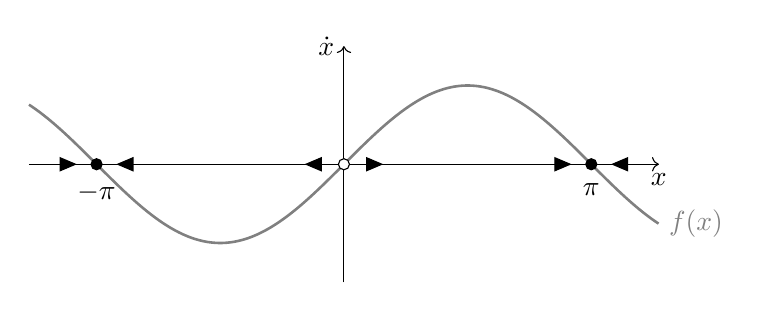
\begin{tikzpicture}[domain=-4:4]

      \draw[->] (-4, 0) -- (4, 0) node[below] {$x$};
      \draw[->] (0, -1.5) -- (0, 1.5) node[left] {$\dot{x}$};

      \draw [variable=\t, domain=-4:4, samples=401, smooth, gray, line width=0.33mm] plot (\t, {sin(\t r)}) node[right] {$f(x)$};

      \node[circle, fill=white, draw=black, inner sep=0pt, minimum size=4pt] (a) at (0, 0) {};

      \node[rotate=90, inner sep=0pt] () at (-0.5, 0) {\tikz\draw[-triangle 45](0, 0) ;};
      \node[rotate=-90, inner sep=0pt] () at (0.5, 0) {\tikz\draw[-triangle 45](0, 0) ;};

      \node[circle, fill=black, draw=black, inner sep=0pt, minimum size=4pt] (a) at (pi, 0) {};

      \node[rotate=-90, inner sep=0pt] () at (pi-0.25, 0) {\tikz\draw[-triangle 45](0, 0) ;};
      \node[rotate=90, inner sep=0pt] () at (pi+0.25, 0) {\tikz\draw[-triangle 45](0, 0) ;};

      \node[circle, fill=black, draw=black, inner sep=0pt, minimum size=4pt] (a) at (-pi, 0) {};

      \node[rotate=-90, inner sep=0pt] () at (-pi-0.25, 0) {\tikz\draw[-triangle 45](0, 0) ;};
      \node[rotate=90, inner sep=0pt] () at (-pi+0.25, 0) {\tikz\draw[-triangle 45](0, 0) ;};

      \node[label={below:$\pi$}] () at (pi, 0) {};
      \node[label={below:$-\pi$}] () at (-pi, 0) {};

    \end{tikzpicture}
  \end{minipage}

  \vspace{1cm}
\end{frame}

\begin{frame}[t, c]{First-order systems}{A motivating example}
  \begin{minipage}{.48\textwidth}
  \end{minipage}%
  \hfill
  \begin{minipage}{.48\textwidth}
  \end{minipage}

  \vspace{1cm}
\end{frame}

\begin{frame}[t, c]{First-order systems}{Examples}
  \begin{minipage}{.48\textwidth}
    \centering
    \begin{circuitikz}
      \draw (0, 0) to[battery1, invert] (0, 3) to [nos] (2.5, 3);
      \draw (2.5, 3) to [R, i>^=$i(t)$, l=$R$] (2.5, 0);
      \draw (2.5, 0) to [C, l=$C$] (0, 0);
    \end{circuitikz}

  \end{minipage}%
  \hfill
  \begin{minipage}{.48\textwidth}
    \centering

    \textbf{Equation :} \( \dot{Q}  = \dfrac{V_0}{RC} - \dfrac{Q}{RC} \)

    \bigskip

    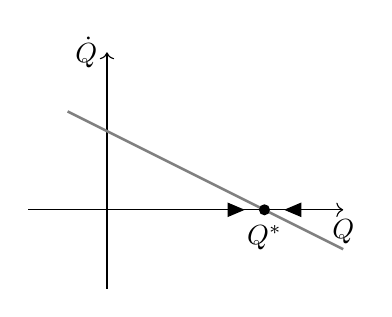
\begin{tikzpicture}[domain=-0.5:3]
      \definecolor{clr1}{RGB}{25.0,84.0,166.0}
      \draw[->] (-1, 0) -- (3, 0) node[below] {$Q$};
      \draw[->] (0, -1) -- (0, 2) node[left] {$\dot{Q}$};

      \draw[gray, line width=0.33mm] plot (\x, {1-0.5*\x});

      \node[circle,fill=black,inner sep=0pt,minimum size=4pt,label=below:{$Q^*$}] (a) at (2, 0) {};

      \node[rotate=90, inner sep=0pt] () at (2.25, 0) {\tikz\draw[-triangle 45](0, 0) ;};
      \node[rotate=-90, inner sep=0pt] () at (1.75, 0) {\tikz\draw[-triangle 45](0, 0) ;};
    \end{tikzpicture}
  \end{minipage}

  \vspace{1cm}
\end{frame}

\begin{frame}[t, c]{First-order systems}{Linear stability}
  \begin{minipage}{.58\textwidth}
    \begin{overprint}
      \onslide<1>
      Let $x^*$ be a fixed point and $\eta = x - x^*$ a small perturbation.
      Then
      %
      \[ \dot{\eta} = \dfrac{d}{dt}(x - x^*) = \dot{x}. \]

      \medskip

      For $\eta$ infinitesimally small, we can write
      %
      \[
      \dot{\eta} = f^{\prime}(x^*) \eta + \mathcal{O}(\eta^2).
      \]

      Neglecting $\mathcal{O}(\eta^2)$, we arrive at the \textbf{linearization of the dynamics about the fixed point} $x^*$.

      \onslide<2>
      The solution is then given by
      %
      \[
      \eta(t) = \exp \left( f^{\prime}(x^*) t \right) \eta_0.
      \]

      Fixed points can be classified based on $\mathrm{sign}\ f^{\prime}(x^*)$.

      \begin{itemize}
      \item If $f^{\prime}(x^*) < 0$, $\eta(t)$ decays exponentially fast.
        The fixed point is said to be \textbf{linearly stable}.

        \medskip

      \item If $f^{\prime}(x^*) > 0$, $\eta(t)$ decays exponentially fast.
        The fixed point is said to be \textbf{linearly unstable}.

        \medskip

      \item If $f^{\prime}(x^*) = 0$, one cannot conclude and nonlinear analyses are required.

      \end{itemize}
    \end{overprint}
  \end{minipage}
  %
  \hfill
  \begin{minipage}{.38\textwidth}
    \centering
    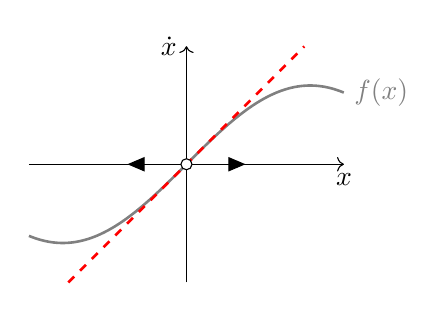
\begin{tikzpicture}[domain=-2:2]

      \draw[->] (-2, 0) -- (2, 0) node[below] {$x$};
      \draw[->] (0, -1.5) -- (0, 1.5) node[left] {$\dot{x}$};

      \draw [variable=\t, domain=-2:2, samples=401, smooth, gray, line width=0.33mm] plot (\t, {sin(\t r))}) node[right] {$f(x)$};
      \draw [variable=\t, domain=-1.5:1.5, samples=401, smooth, red, line width=0.33mm, dashed] plot (\t, {\t});

      \node[circle, fill=white, draw=black, inner sep=0pt, minimum size=4pt] (a) at (0, 0) {};

      \node[rotate=90, inner sep=0pt] () at (-0.75, 0) {\tikz\draw[-triangle 45](0, 0) ;};
      \node[rotate=-90, inner sep=0pt] () at (0.75, 0) {\tikz\draw[-triangle 45](0, 0) ;};

    \end{tikzpicture}
  \end{minipage}

  \vspace{1cm}
\end{frame}

\begin{frame}[t, c]{First-order systems}{Some cavats : Finite-time blow up}
  \begin{minipage}{.63\textwidth}
    Consider the system $\dot{x} = 1 + x^2$ with initial condition $x(0) = 0$.
    Its solution is given by
    %
    \[
    \begin{aligned}
      \int \dfrac{dx}{1+x^2} & = \int dt \\
      \tan^{-1} x & = t + C \\
      x(t) = \tan t.
    \end{aligned}
    \]

    As $t \to \pm \nicefrac{\pi}{2}$, $x(t) \to \pm \infty$.
    The system has solutions reaching infinity \emph{in finite time}.
    This phenomenon is called \textbf{blow-up} and is relevant in e.g.\ combustion models.
  \end{minipage}%
  \hfill
  \begin{minipage}{.33\textwidth}
    \begin{overprint}
      \onslide<1>
      \centering
      \begin{tikzpicture}[domain=-2:2]
        
        \draw[->] (-2, 0) -- (2, 0) node[below] {$x$};
        \draw[->] (0, -1) -- (0, 5) node[left] {$\dot{x}$};
        
        \draw [variable=\t, domain=-1.75:1.75, samples=401, smooth, gray, line width=0.33mm] plot (\t, {1 + \t*\t}) node[right] {$f(x)$};

      \end{tikzpicture}

      \onslide<2>
      \centering
      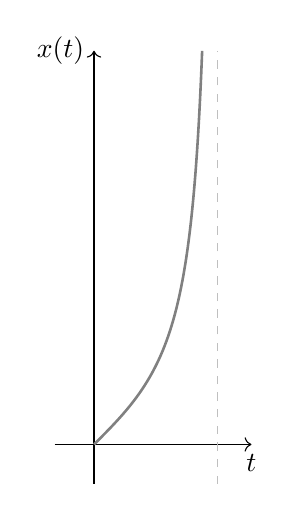
\begin{tikzpicture}[domain=0:2]
        
        \draw[->] (-0.5, 0) -- (2, 0) node[below] {$t$};
        \draw[->] (0, -0.5) -- (0, 5) node[left] {$x(t)$};
        
        \draw [variable=\t, domain=0:1.3734, samples=401, smooth, gray, line width=0.33mm] plot (\t, {tan(\t r)});

        \draw[dashed, lightgray] (pi/2, -0.5) -- (pi/2, 5) {};

      \end{tikzpicture}

    \end{overprint}
  \end{minipage}

  \vspace{1cm}
\end{frame}

\begin{frame}[t, c]{First-order systems}{Some caveats : Non-uniqueness of the solution}
  \begin{minipage}{.68\textwidth}
    Consider the system $\dot{x} = \sqrt[3]{x}$ with initial condition $x(0) = 0$.
    $x=0$ is obviously a fixed point and so $x(t) = 0$ is the solution. But is it ?

    \[
    \begin{aligned}
      \dfrac{dx}{dt} & = \sqrt[3]{x} \\
      \int \dfrac{dx}{\sqrt[3]{x}} & = \int dt \\
      \dfrac{3}{2} x^{\nicefrac{2}{3}} & = t + C
    \end{aligned}
    \]

    Given that $x(0) = 0$, then $x(t) = \left( \dfrac{2}{3} t \right)^{\nicefrac{3}{2}}$ is also solution !
  \end{minipage}%
  \hfill
  \begin{minipage}{.28\textwidth}
    \centering
    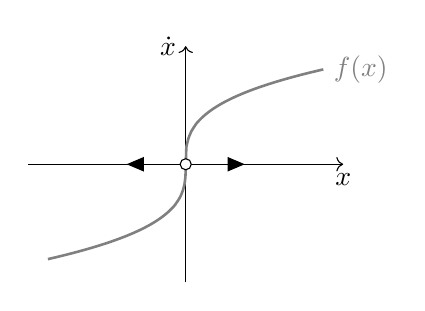
\begin{tikzpicture}[domain=-2:2]

      \draw[->] (-2, 0) -- (2, 0) node[below] {$x$};
      \draw[->] (0, -1.5) -- (0, 1.5) node[left] {$\dot{x}$};

      \draw [variable=\t, domain=-1.75:1.75, samples=401, smooth, gray, line width=0.33mm] plot (\t, {\t^(1/3)}) node[right] {$f(x)$};

      \node[circle, fill=white, draw=black, inner sep=0pt, minimum size=4pt] (a) at (0, 0) {};

      \node[rotate=90, inner sep=0pt] () at (-0.75, 0) {\tikz\draw[-triangle 45](0, 0) ;};
      \node[rotate=-90, inner sep=0pt] () at (0.75, 0) {\tikz\draw[-triangle 45](0, 0) ;};

    \end{tikzpicture}
  \end{minipage}

  \vspace{1cm}
\end{frame}

\begin{frame}[t, c]{First-order systems}{Impossibility of oscillations}
  \begin{block}{\centering \textbf{Warning}}
    \centering
    First-order systems defined on the real number line cannot exhibit oscillatory behaviour !
  \end{block}

  \vspace{0.5cm}

  \begin{minipage}{.38\textwidth}
    Trajectories of first-order systems can only vary monotically.
    They either end up on a stable fixed point or diverge to $\pm \infty$.
  \end{minipage}%
  \hfill
  \begin{minipage}{.58\textwidth}
    \centering
    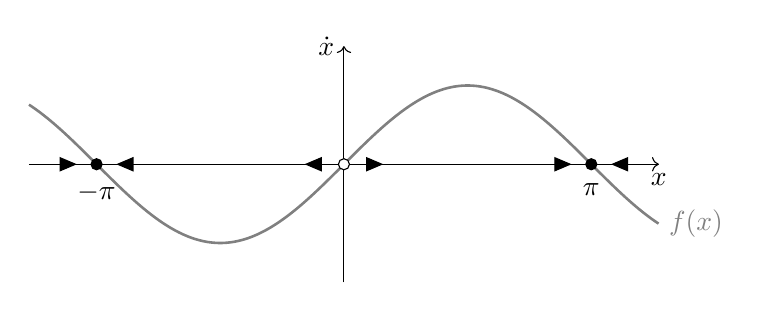
\begin{tikzpicture}[domain=-4:4]

      \draw[->] (-4, 0) -- (4, 0) node[below] {$x$};
      \draw[->] (0, -1.5) -- (0, 1.5) node[left] {$\dot{x}$};

      \draw [variable=\t, domain=-4:4, samples=401, smooth, gray, line width=0.33mm] plot (\t, {sin(\t r)}) node[right] {$f(x)$};

      \node[circle, fill=white, draw=black, inner sep=0pt, minimum size=4pt] (a) at (0, 0) {};

      \node[rotate=90, inner sep=0pt] () at (-0.5, 0) {\tikz\draw[-triangle 45](0, 0) ;};
      \node[rotate=-90, inner sep=0pt] () at (0.5, 0) {\tikz\draw[-triangle 45](0, 0) ;};

      \node[circle, fill=black, draw=black, inner sep=0pt, minimum size=4pt] (a) at (pi, 0) {};

      \node[rotate=-90, inner sep=0pt] () at (pi-0.25, 0) {\tikz\draw[-triangle 45](0, 0) ;};
      \node[rotate=90, inner sep=0pt] () at (pi+0.25, 0) {\tikz\draw[-triangle 45](0, 0) ;};

      \node[circle, fill=black, draw=black, inner sep=0pt, minimum size=4pt] (a) at (-pi, 0) {};

      \node[rotate=-90, inner sep=0pt] () at (-pi-0.25, 0) {\tikz\draw[-triangle 45](0, 0) ;};
      \node[rotate=90, inner sep=0pt] () at (-pi+0.25, 0) {\tikz\draw[-triangle 45](0, 0) ;};

      \node[label={below:$\pi$}] () at (pi, 0) {};
      \node[label={below:$-\pi$}] () at (-pi, 0) {};

    \end{tikzpicture}
  \end{minipage}
  
  \vspace{2cm}
\end{frame}

\end{document}
